%
% Documento: Introdução
%

\chapter{Controle de Sistemas Não Lineares}
\label{chap:sistemas-nao-lineares}

O controle de sistemas não lineares tem sido alvo de extensiva pesquisa. Nos capítulos seguintes, este tema será abordado com maior profundidade. Nesta seção, é mostrada  uma visão geral sobre sistemas não lineares e a relação deles com o projeto aqui proposto.

Segundo \citeonline[p.~2]{Dorf2011}, um sistema de controle é a interconexão de componentes formando uma configuração que fornecerá uma resposta desejada dele. Ainda segundo o autor, seu controle adequado permite o desenvolvimento de produtos viáveis úteis para a sociedade. Para tanto, os dois objetivos, que são a compreensão e o controle dos sistemas, são complementares porque o controle eficaz deles requer que o sistema seja compreendido e modelado.

Este trabalho consiste na implementação de um controle para um quadrotor que é, também, um sistema não linear. Para contextualizar este tipo de sistema, será abordado, neste capítulo, além do quadrotor, o sistema de pêndulo invertido, que é um dos principais alvos de estudo dentre os sistemas instáveis não lineares, sendo comumente usado em \textit{benchmarks} para verificar a eficácia de métodos de controle \cite{Arai2014}.

%\cite{Dorf2011}
%\cite{Ogata2010}
%\section{Analogia do Sistema Usando o Pêndulo Invertido}
%\label{sec:sistemas-inverted-pendulum}

%Um sistema de pêndulo invertido consiste em uma haste suspensa verticalmente sobre um carro motorizado, como mostrado na Figura \ref{fig:diagrama-pendulo-invertido}. O objetivo do controle de atitude, que é referente ao controle de orientação angular, é manter a haste na posição vertical mesmo após o sistema sofrer alguma perturbação. Como o pêndulo invertido é um sistema instável, após sofrer esta perturbação a haste deverá cair a menos que uma ação de controle adequada seja exercida.

Neste exemplo, é considerado um problema bidimensional, em que o pêndulo se move apenas para a direita e para esquerda (i.e.\ no plano da página), mas não para frente e para trás (i.e\ no plano ortogonal a ela). Outra simplificação feita é a consideração de que o centro de gravidade da haste do pêndulo seja seu centro geométrico.

%\begin{figure}[!htb]
%    \centering
%    \caption{Diagrama do sistema de pêndulo invertido; (a) sistema de pêndulo invertido; (b) diagrama de corpo livre}
%    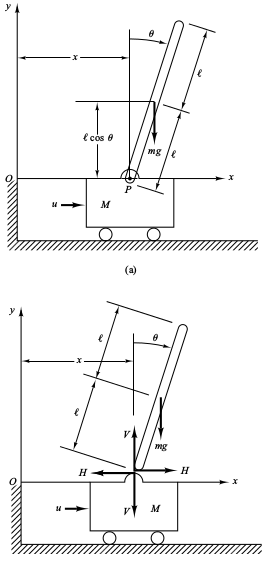
\includegraphics[width=0.55\textwidth]{./04-figuras/Ogata2010_inverted_pendulum_diagram_complete}
%    \fonte{\citeonline[p.~69]{Ogata2010}}
%    \label{fig:Ogata2010_inverted_pendulum_diagram_complete}
%\end{figure}
\begin{figure}[!htb]
    \centering
    \caption{Diagrama do sistema de pêndulo invertido}
    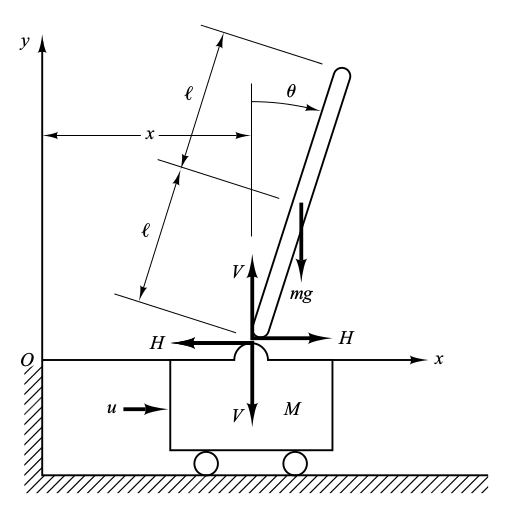
\includegraphics[width=0.6\textwidth]{./04-figuras/sistemas-nao-lineares/diagrama-pendulo-invertido}
    \fonte{Adaptado de \citeonline[p.~69]{Ogata2010}}
    \label{fig:diagrama-pendulo-invertido}
\end{figure}
%diagrama-pendulo-invertido

Além disso, o sistema mostrado na Figura \ref{fig:diagrama-pendulo-invertido}, assume que uma força $u$ seja aplicada ao carro, considerando $M$ como a massa do carro, $m$ a massa da haste, $g$ a força da gravidade, $x$ o deslocamento no eixo horizontal, $l$ a metade do comprimento da haste, $\theta$ o ângulo da haste com relação ao eixo vertical, $P$ o ponto de rotação do pêndulo sobre o carro, $H$ o movimento horizontal do centro de gravidade da haste do pêndulo e $V$ o movimento vertical do centro de gravidade da haste do pêndulo.

Com estes parâmetros, \citeonline[p.~69]{Ogata2010} mostra que o sistema descrito pode ser representado da seguinte maneira  no espaço de estados:
\begin{center}\label{eq:k1}
$\dot{x}=Ax+Bu$ \\
$y=Cx+Du$
\end{center}
em que:
%\begin{equation*}
%x=
%\left[ \begin{array}{@{}*{4}{c}@{}}
%     \theta & \dot{\theta} & x & \dot{x} \\
%\end{array} \right]^T
%\end{equation*}
%
%Além disto, o vetor $y$ de saída do sistema foi definido como:
\[
%	x =
%	\begin{bmatrix}
%	\theta & \dot{\theta} & x & \dot{x}
%	\end{bmatrix}^T\quad
	x =
		\begin{bmatrix}
		\theta \\ \dot{\theta} \\ x \\ \dot{x}
		\end{bmatrix}\quad
	y = 
	\begin{bmatrix}
			\theta \\
			x
	\end{bmatrix}
\]
\[
	A = 
	\begin{bmatrix}
		0 & 1 & 0 & 0 \\
		\frac{M+m}{Ml}g & 0 & 0 & 0 \\
		0 & 0 & 0 & 1 \\
		-\frac{m}{M}g & 0 & 0 & 0
	\end{bmatrix}\quad
	B = 
	\begin{bmatrix}
		0 \\
		-\frac{1}{Ml} \\
		0 \\
		\frac{1}{Ml}
	\end{bmatrix}
\]

\[
	C = 
		\begin{bmatrix}
			1 & 0 & 0 & 0 \\
			0 & 0 & 1 & 0
		\end{bmatrix}\quad
	D = 
		\begin{bmatrix}
			0 \\
			0
		\end{bmatrix}
\]

Como o sistema de pêndulo invertido não é o foco deste trabalho, sendo referenciado apenas como uma analogia para sistemas não-lineares instáveis, o desenvolvimento da modelagem matemática mostrado por \citeonline[p.~70]{Ogata2010} não foi explicitado.

Uma vez exibido um modelo de um sistema instável mais simples, pode-se melhor compreender a modelagem de um sistema mais complexo como é o de um quadrotor, assunto este que é abordado na próxima seção.
%Desta forma, se obtém a representação completa do sistema de pêndulo invertido no espaço de estados.
%Este sistema foi modelado por \citeonline[p.~69]{Ogata2010}
%\hl{Inserir diagrama de blocos do sistema}\\

%\section{Quadricóptero}
%\label{sec:sistemas-quadcopter}

Como definido no \autoref{chap:introducao}, um quadricóptero é uma aeronave cuja propulsão é obtida a partir do uso de quatro rotores. O diagrama de um quadrotor é mostrado na \autoref{fig:drone_diagram}. Neste diagrama, $x$, $y$ e $z$ indicam a orientação dos eixos, $F_1$, $F_2$, $F_3$ e $F_4$ são as forças geradas pela propulsão de cada um dos motores. As variáveis $\phi$, $\theta$, e $\psi$ são os ângulos de rotação do quadricóptero em relação aos eixos $x$, $y$ e $z$ respectivamente. Estes ângulos são também chamados ângulos de \textit{roll} (arfagem), \textit{pitch} (rolamento) e \textit{yaw} (guinada), respectivamente. Além disto, o diagrama mostra ainda o sentido de rotação de cada um dos quatro rotores. Como se pode ver, os rotores dispostos sobre um mesmo eixo possuem um mesmo sentido de rotação. Desta forma, os rotores 1 e 3 (dispostos sobre o eixo $x$), giram no sentido horário. Já os rotores 2 e 4 (dispostos sobre o eixo $y$) giram no sentido anti-horário. Esta disposição dos rotores permite que os empuxos horizontais se anulem, possibilitando a estabilidade do quadricóptero.

\begin{figure}[!htb]
    \centering
    \caption{Diagrama de um quadricóptero}
    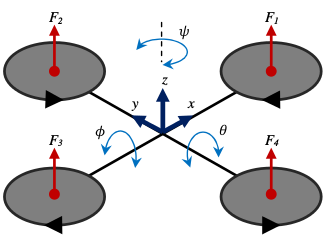
\includegraphics[width=0.5\textwidth]{./04-figuras/drone_diagram/drone_diagram_20}
    \fonte{\citeonline[p.~1]{Ariffanan2014}}
    \label{fig:drone_diagram}
\end{figure}

Os dois aspectos diferentes para se controlar sobre um quadrotor são: a sua altitude, ou seja, seu posicionamento vertical (posição sobre o eixo $z$); e a sua atitude, que é referente à devida orientação angular do \textit{drone}, ou seja, obter os devidos valores para $\theta$, $\phi$ e $\psi$. 



%\cite{Balas2007}.
%\cite{Goodwin2001}.
%\subsection{Instabilidade do Sistema}
%\label{subsec:sistemas-quadcopter-instability}
%Caracterização da instabilidade, por zeros e pólos.
